\chapter{シミュレーション天文学}

\section{シミュレーション天文学とは}
天文学と聞くと,望遠鏡で星を観測して云々,というイメージしか湧かないかもしれないが,最近の天文学というのは,実際に天体観測を行うもの
\footnote{実際に天体観測を行う天文学の中にも,目に見える可視光のほかに,赤外線を使って観測を行う赤外線天文学,X線を使うX線天文学,電波を使う電波天文学,最近では,ニュートリノを使ったニュートリノ天文学というものもある.}
の他に,天体の運動や構造などの理論を考える理論天文学,そして,今回取り上げるような,天体のシミュレーションをするシミュレーション天文学など,様々な分野がある.


特に,シミュレーション天文学は,惑星の形成,銀河の衝突,ブラックホールの降着円盤,銀河の衝突,宇宙の大規模構造など,実際に観測することが難しい,もしくは観測できていても,それを確実に説明する理論がなかったり,計算量が膨大になったりするもののシミュレーションを行う.

国立天文台の4D2Uのウェブサイトなどを見ると,最新のシミュレーション天文学の成果を見ることができる.

\section{N体シミュレーション}
さて,このようにさまざまな天文現象を扱うシミュレーション天文学だが,これらのシミュレーションは,実際にはどのように行っているのだろうか.
ここでは,シミュレーション天文学の一分野であるN体シミュレーションについて考えてみよう.


N体シミュレーションというのは,その名の通り,N個
\footnote{Nは任意の自然数}
の物体の運動をシミュレーションするもので,多体シミュレーションとも呼ばれる.


天文学でN体シミュレーションが用いられる分野としては,惑星形成理論などがある.

実は,現在の太陽系がどのように形成されたかということには謎が多く,様々な形成シナリオが提案されているが,いったいどれが正しいのか,ということは中々検証できるものではない.
\footnote{シミュレーション以外での検証アプローチとして,太陽系形成初期の物質を調べる,というものがある.しかし,地球にある物質は熱変性や風化を受けているため,太陽系形成初期そのままの物質は全く残っていない.そのため,熱変性や風化を受けていない小惑星のサンプルを入手しよう,という試みが,あの「はやぶさ」である.}

そのため,微惑星をコンピューター上で様々な条件で衝突,合体させ,現在の太陽系の形成の条件を探る,というのが惑星形成のシミュレーションであり,これはたくさんの微惑星の運動を計算しなければならないので,N体シミュレーションの一種である.

\section{2体問題}
さて,N体シミュレーションでは,N個の天体の運動を考えるわけだが,急にたくさんの天体の運動を考えるのは大変なので,まずは2つの天体の運動について考えてみよう.
\begin{figure}[htbp]
\centering
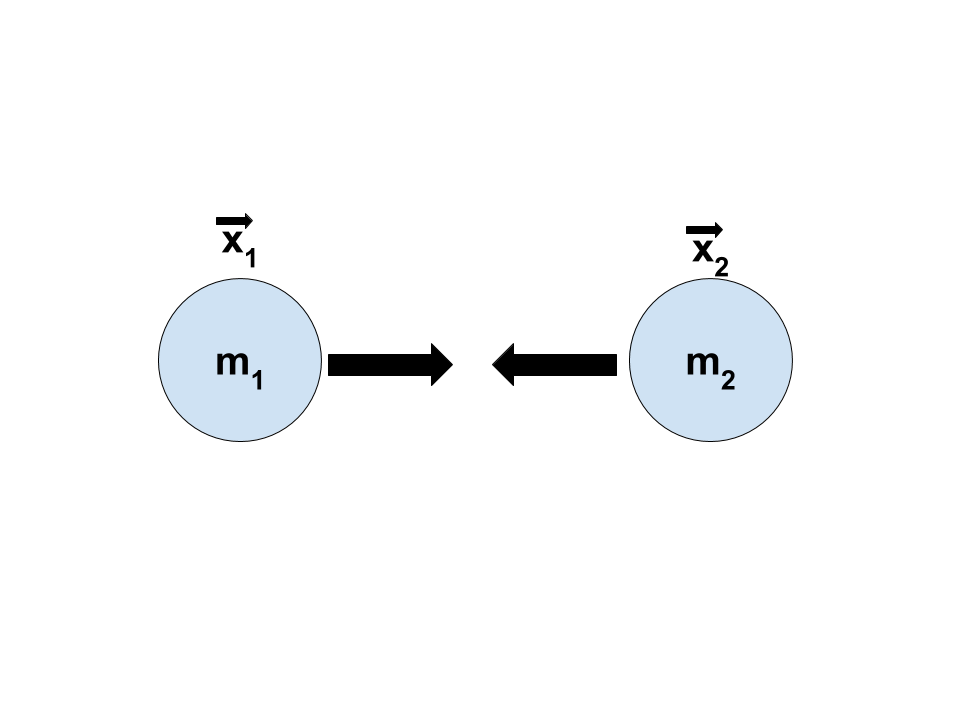
\includegraphics[width=6cm]{img/2body.png}
\caption{2つの天体が,互いに万有引力で引き合っている}
\end{figure}
2つの天体は,互いに万有引力で引っ張り合っている.
万有引力の強さは,2つの天体の質量と距離の逆2乗に比例するので,
2つの天体の質量をそれぞれ$m_1,m_2$,位置ベクトルを$\vec{x_1},\vec{x_2}$とおくと,
それぞれの天体に働く万有引力を$F_1,F_2$は
\begin{align}
F_1 = - \dfrac{G m_1 m_2}{||\vec{x_1}-\vec{x_2}||^2} \dfrac{\vec{x_1}-\vec{x_2}}{||\vec{x_1}-\vec{x_2}||} \\
F_2 = - \dfrac{G m_1 m_2}{||\vec{x_2}-\vec{x_1}||^2} \dfrac{\vec{x_2}-\vec{x_1}}{||\vec{x_2}-\vec{x_1}||}
\end{align}
となる.

よって,天体同士の衝突を考えないとすると,天体にはたらく力は万有引力のみなので,
それぞれ運動方程式を立てると,
\begin{align}
m_1 \dfrac{d^2\vec{x_1}}{dt^2} = - \dfrac{G m_1 m_2}{||\vec{x_1}-\vec{x_2}||^2} \dfrac{\vec{x_1}-\vec{x_2}}{||\vec{x_1}-\vec{x_2}||} \\
m_2 \dfrac{d^2\vec{x_2}}{dt^2} = - \dfrac{G m_1 m_2}{||\vec{x_2}-\vec{x_1}||^2} \dfrac{\vec{x_2}-\vec{x_1}}{||\vec{x_2}-\vec{x_1}||}
\end{align}
となる.
両辺を$m_1,m_2$でわって,
\begin{align}
\dfrac{d^2\vec{x_1}}{dt^2} = - \dfrac{G m_2}{||\vec{x_1}-\vec{x_2}||^2} \dfrac{\vec{x_1}-\vec{x_2}}{||\vec{x_1}-\vec{x_2}||} \\
\dfrac{d^2\vec{x_2}}{dt^2} = - \dfrac{G m_1}{||\vec{x_2}-\vec{x_1}||^2} \dfrac{\vec{x_2}-\vec{x_1}}{||\vec{x_2}-\vec{x_1}||}
\end{align}
$\vec{r} = \vec{x_1} - \vec{x_2}$,$r = ||\vec{x_1} - \vec{x_2}||$とおくと,
この2式の差は
\begin{align}
\dfrac{d^2}{dt^2} (\vec{x_1} - \vec{x_2}) = - G (m_1+M_2) \dfrac{\vec{r}}{r^3}
\end{align}
となる.
これは2つの天体の相対運動を考えることに等しい.
詳細は省略するが,この式を積分し,$r$についての微分方程式を解くと,これが楕円軌道を描くことが分かる.
\footnote{僕はまだ面積速度一定の法則を導くところまでしか理解できていない...今年中には理解したいところ.}

\section{N体問題の数値的解法}
ということで,$N=2$のとき,つまり,「2体問題」は解析的に解くことができるのだが,$N>2$のときはそうもいかなくなってくる.
$N=3$のとき,つまり「3体問題」のときについては,一部の条件を満たす有名な問題
\footnote{1つだけ質量がとても小さい,など}
の時に限っては解くことができるが,基本的には$N>2$のときは解析的に解くことは不可能である.


そこで,数値計算が用いられるのだ.
多体系での重力で相互作用する粒子の運動方程式は,2体問題の時と似ていて,
\begin{align}
\dfrac{d^2 \vec{x_i}}{dt^2} = - \sum_{j\neq i} G m_j \dfrac{\vec{x_j} - \vec{x_i}}{||\vec{x_j} - \vec{x_i}||^3}
\label{nbody}
\end{align}
というようになる.
ようするに,自分以外の他すべての天体との重力相互作用の和を考えるのだ.
N体シミュレーションでは,式\ref{nbody}を直接数値積分することにより,多体系の時間発展を計算する.

\newpage
数値計算は他の章を参考にしてもらうとして,これを実際にやり,POV-Rayでレンダリングしてみると,図\ref{nbody-cg}のような結果が得られた.
\begin{figure}
\centering
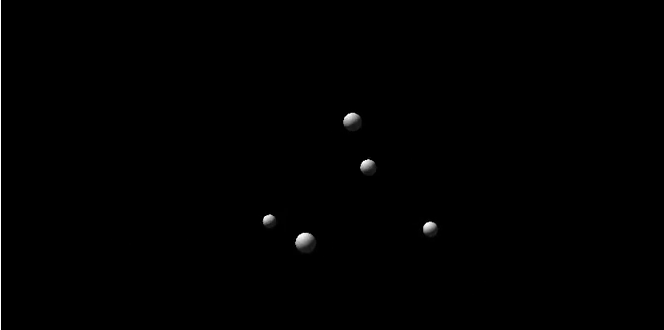
\includegraphics[width=10cm]{img/nbody-cg.png}
\caption{実際にN体シミュレーションをやってみた結果}
\end{figure}
しかし,このシミュレーションでは数値積分にオイラー法を用いており,精度が低く,刻み幅制御もできないので,すぐに計算が破綻してしまう.
そのため,今後はそれらの点を改善していこうと思っている.
このシミュレーションのソースコードは\url{https://github.com/asanotigaku/planet}に置いてあるので,よかったら見てみてほしい.
